\documentclass{article}

\usepackage{fancyhdr}
\usepackage{listings}
\usepackage{xcolor}
\usepackage{hyperref}
\usepackage{graphicx}

\title{CSC 648 Homework 4: MLP For Regression}
\date{Due: Tuesday Oct 8, at 11:59 PM, 2024}
\author{Miguel Antonio Logarta}

\pagestyle{fancy}

\fancyhead[L]{SFSU, CSC 648}  % Left side of the header
\fancyhead[C]{Fall 2024}  % Center of the header
\fancyhead[R]{Due: Tuesday Oct 8, 2024}  % Right side of the header (current date)

% Set up the style for Python code
\lstset{
    language=Python,
    basicstyle=\ttfamily\small,
    keywordstyle=\color{blue}\bfseries,
    commentstyle=\color{gray}\itshape,
    stringstyle=\color{red},
    showstringspaces=false,
    numbers=left,  % Line numbers on the left
    numberstyle=\tiny\color{gray},
    frame=single,  % Draw a frame around the code
    breaklines=true,  % Line breaking for long code lines
}

\begin{document}

\maketitle  % This command generates the title page.
\thispagestyle{fancy}

\section{Introduction}
For this homework assignment, we are tasked with fitting a \underline{nonlinear} regression curve using a Multilayer Perceptron. It requires prior knowledge from making a Linear Regression curve in a previous exercise and using an MLP to classify a XOR dataset in another exercise. 
\section{Loading the Data}
For our data, we have to read in a csv file called \textit{mlp\_regression\_data.csv}. In it contains two columns \textit{x}, and \textit{y}. Using pandas, I loaded the data into a dataframe. This will make it easier for me to normalize and load my data into the dataset later. 

Since the assignment does not require us to split the data into training, validation, and, testing datasets, I just took the entire dataset and assigned it to \textit{X\_train} and \textit{y\_train}.

\begin{lstlisting}
    # Load the data from csv file
    df = pd.read_csv('mlp_regression_data.csv')

    # Convert to numpy arrays
    X = df["x"].values # Features (Only 1 feature)
    y = df["y"].values # Labels (Only 1 class)

    # Set our training data
    X_train = X
    y_train = y
\end{lstlisting}

I also modified \textit{MyDataset()} class to transform \textit{X} and \textit{y} from pandas dataframes into Torch Tensors. I learned that the code also transforms \textit{X} and \textit{y} from 1 dimensional array, into a 2 dimensional array with 1 column. This helped greatly when it came to training the model.

\begin{lstlisting}
# Data loader
class MyDataset(Dataset):
    def __init__(self, X, y):
        self.features = torch.tensor(X, dtype=torch.float32)
        self.features = self.features.view(-1,1) # Turn this into a 2D tensor with 1 column

        self.labels = torch.tensor(y, dtype=torch.float32)
        self.labels = self.labels.view(-1, 1)

    def __getitem__(self, index):
        x = self.features[index]
        y = self.labels[index]        
        return x, y

    def __len__(self):
        return self.labels.shape[0]
\end{lstlisting}

\begin{lstlisting}
    # Load training data
    train_ds = MyDataset(X_train, y_train)

    # Load dataset into dataloader
    train_loader = DataLoader(
        dataset=train_ds,
        batch_size=32,
        shuffle=True,
    )
\end{lstlisting}

\section{MLP Model}
For my MLP Model, there were multiple things to configure. We only have 1 feature and 1 class. For my 3 hidden layers, I had 50 neurons for my first layer, then 100 for my second layer.

For my activation function, I learned that we had three activation functions from class. We have sigmoid, Linear Activation, and ReLU. Sigmoid is best for binary classification problems, but that isn't the probelm we're solving here. A linear activiation function seems to be the best sinec its goal is to predict a continous value (which is \textit{y} in this case). ReLU is the same, however, it is for problems where the output is non-negative.

Since I know that our data is continous and our output data is non-negative, I chose ReLU as my activiation function.
\begin{lstlisting}
# Our MLP Model
class MLP(torch.nn.Module):
    def __init__(self, num_features, num_classes):
        super().__init__()

        self.all_layers = torch.nn.Sequential(
            # 1st hidden layer
            torch.nn.Linear(num_features, 50),
            # torch.nn.Sigmoid(),
            torch.nn.ReLU(),

            # 2nd hidden layer
            torch.nn.Linear(50, 100),
            # torch.nn.Sigmoid(),
            torch.nn.ReLU(),

            # output layer
            torch.nn.Linear(100, num_classes),
        )

    def forward(self, x):
        logits = self.all_layers(x)
        return logits
\end{lstlisting}

\section{Training Loop}
Here is my training loop. I am using the mse\_loss() function. In the loop, I also computed the loss per batch and took the average of those losses into our epoch loss.

\begin{lstlisting}
    # Begin training loop
    torch.manual_seed(123)
    model = MLP(num_features=1, num_classes=1) # 1 input neuron 1 output neuron
    optimizer = torch.optim.SGD(model.parameters(), lr=0.1) # Stochastic gradient descent

    num_epochs = 200
    losses = []

    for epoch in range(num_epochs):
        running_loss = 0.0
        model = model.train()
        for batch_idx, (features, labels) in enumerate(train_loader):
            
            # Forward pass
            logits = model(features)
            loss = F.mse_loss(logits, labels) # Loss function
            
            # Backwards pass
            optimizer.zero_grad()
            loss.backward()

            # Update model parameters
            optimizer.step()

            # Log the loss
            running_loss += loss.item()
            print(f'Epoch: {epoch+1:03d}/{num_epochs:03d}'
                f' | Batch {batch_idx+1:03d}/{len(train_loader):03d}'
                f' | Loss: {loss:.2f}')
        
        # Divide the total running loss of the epoch by the size of the batch
        losses.append(running_loss / len(train_loader))
        
\end{lstlisting}
\section{Normalizing the Data}
Early on, I realized that not normalizing my data caused significant issues with my loss function. For example, when I was using ReLU, the loss would quickly spiral out of control and go to infinity. It caused the value of the loss to become NaN. So before, I plugged the data into the model, I normalized the data like so:
\begin{lstlisting}
    # Normalize training data
    X_mean = X_train.mean(axis=0)
    X_std = X_train.std(axis=0)
    y_mean = y_train.mean(axis=0)
    y_std = y_train.std(axis=0)

    X_train = (X_train - X_mean) / X_std
    y_train = (y_train - y_mean) / y_std
\end{lstlisting}

This fixed my problems with the loss function

\section{Plotting the data points}
Using matplotlib, I had three separate functions to plot the original data points, the nonlinear regression curve, and the loss as a function of epoch

\begin{lstlisting}
    
def plot_original_data(X, y):
    plt.title("Multi Layer Perception (MLP)")
    plt.scatter(X, y, s=3, label="Original Data")
    plt.xlabel("x")
    plt.ylabel("y")


def plot_decision_boundary(X, y, X_train, model, step=0.01):
    # Get data points
    X_range = torch.arange(X_train.min(), X_train.max(), step).view(-1, 1)
    y_pred = model(torch.tensor(X_range, dtype=torch.float32)).detach().numpy()

    X_mean = X.mean(axis=0)
    X_std = X.std(axis=0)
    y_mean = y.mean(axis=0)
    y_std = y.std(axis=0)

    # Denormalize
    X_range = (X_range*X_std)+X_mean
    y_pred = (y_pred*y_std)+y_mean

    plt.plot(X_range, y_pred, color='orange', label='Regression Curve', linewidth=3)


def plot_training_loss(loss):
    plt.title("Training Loss")
    plt.xlabel("Epochs")
    plt.ylabel("Loss")
    plt.plot(range(1, len(loss) + 1), loss, label="Training Loss")
    plt.show()
\end{lstlisting}

\begin{lstlisting}
    # Plot training results
    plot_original_data(X, y)
    plot_decision_boundary(X, y, X_train, model, step=0.01)
    plt.show()

    # Plot the training loss
    plot_training_loss(losses)
\end{lstlisting}

Here are my results:

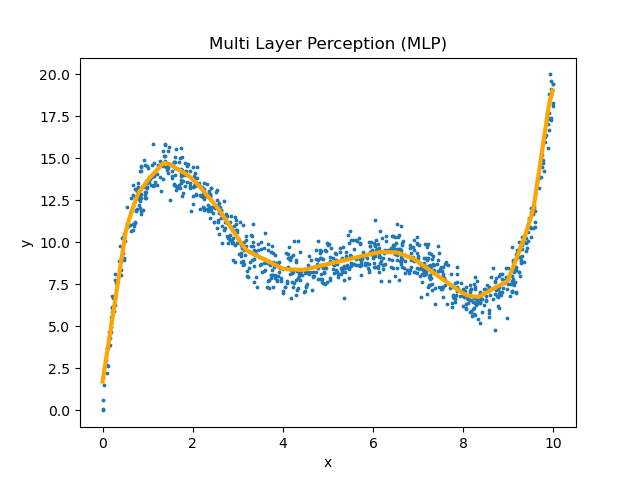
\includegraphics[width=120mm]{Figure_1.png}
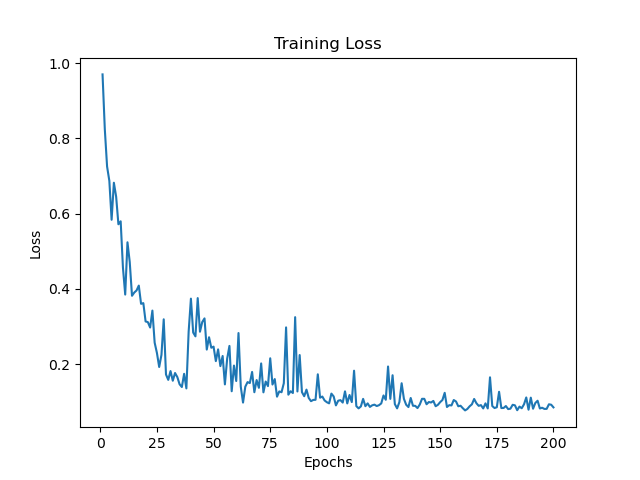
\includegraphics[width=120mm]{Figure_2.png}

\section{Hyper Parameters}
I also played with some of the hyper parameters. The most interesting thing I found was how changing ReLU to Sigmoid made the regression line really inaccurate.

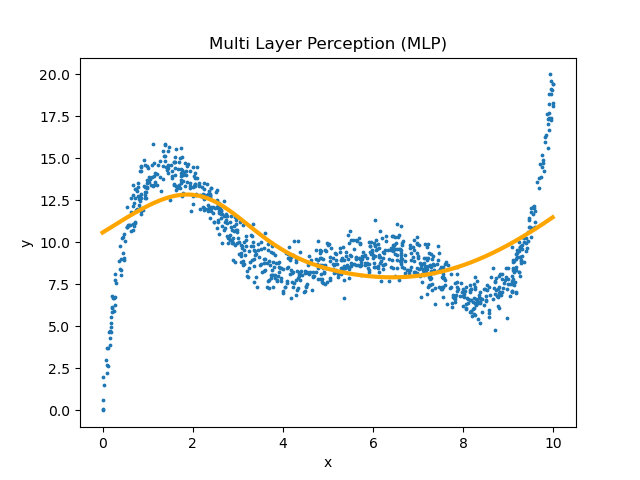
\includegraphics[width=120mm]{Figure_3.png}
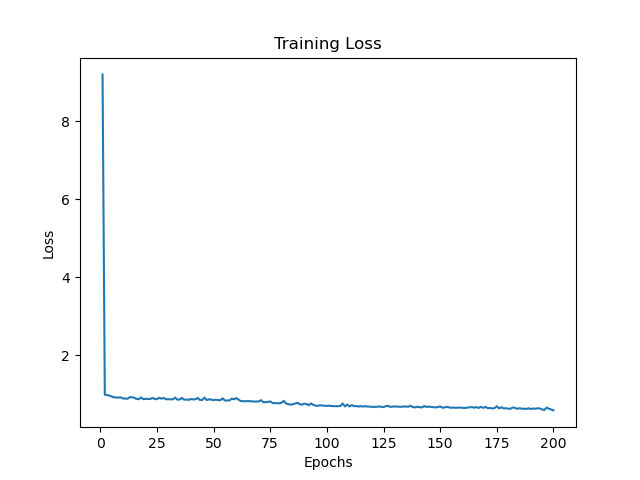
\includegraphics[width=120mm]{Figure_4.png}

\end{document}
